This element simulates a commonplace type of aperture restriction, consisting of a
bump on one or both sides of a chamber. The parameters of the speedbump are
illustrated in Fig. \ref{fig:speedbump}
It may be useful to know that the radius $R$ of the cylinder from which the
speedbump is made is
\begin{equation}
  R = \frac{C^2 + 4 h^2}{8 h},
\end{equation}
where $C$ is the chord length and $h$ is the bump height.
Solving for $h$, we have
\begin{equation}
h = R - \sqrt{R^2 - \left(\frac{C}{2}\right)^2}.
\end{equation}

\begin{figure}[htb]
\center
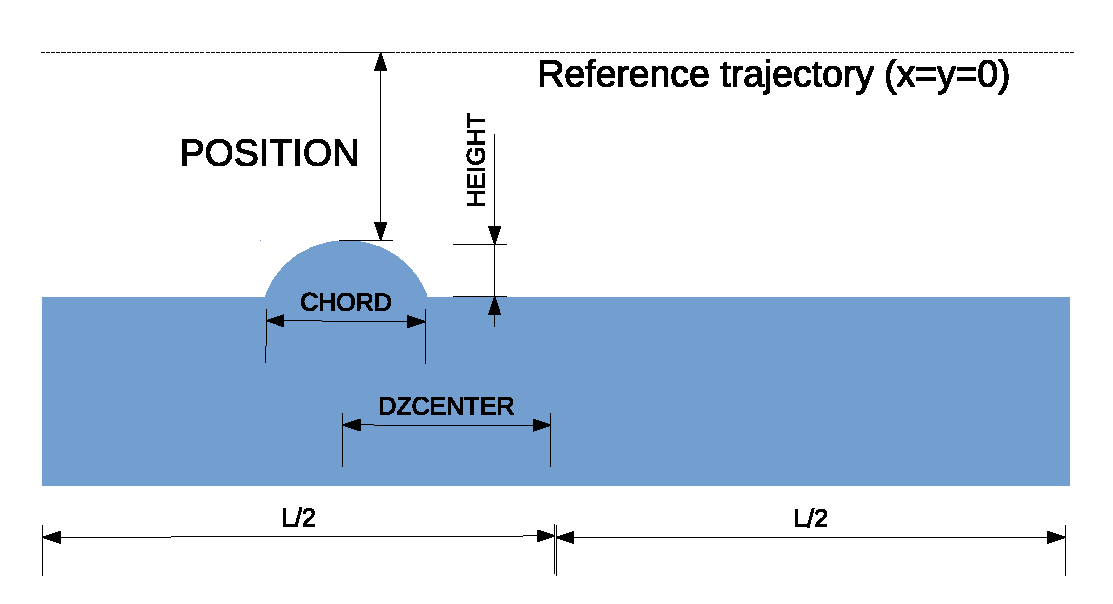
\includegraphics[width=0.8\linewidth]{speedbump}
\caption{Illustration of the parameters used in specifying a speedbump.}
\label{fig:speedbump}
\end{figure}

\clearpage
